\chapter{Modelling The Energy Usage Of Ethereum}
\label{Modelling}

% ____________________________________________________________________________
\section{Summary}

This chapter constitutes the technical section of this study, comprising of creating our mathematical model to estimate the energy consumption of PoS Ethereum, called 'Model-A', and then gathering data to implement that model amongst others for comparative analysis. 
% ____________________________________________________________________________

% %  Model-AAAAAAAAAAAAAAAAAAAAAAAAAAAAAAAAAAAAAAAAAA
% \subsection{Model-A}
% From the research,it seems like power usage is usually not the limiting factor but rather the storage space needed to run validators.

% The recommended hardware for a validator one is shown in table \_\_ of the appendix as well as in the table below. \_\_

% So according to this hardware recommendation, we could estimate the power usage depending on statistics provided by manufacturers. Let's assume the same configuration of hardware as in the \cite{CryptoCarbonRatingsInstitute2022TheNetwork} (They don't mention type of power supply and mainboard).  According to data from the manufacturers, the power consumption for this configuration comes out to the following: 

% \begin{itemize}
%     \item Processor TDP - 105W
    
%     \item An SSD uses 5W while Active
    
%     \item Every 8GB of memory uses 3W, so 16GB of memory will use 6W
    
%     \item For a solo validator set-up (non-specialised hardware), miscellaneous components are likely to use another 30W
    
%     \item As 92\% efficiency is common, the machine will likely peak at 178W of AC power drawn from the wall
    
%     \item The machine will run at idle power consumption 50-90\% of time, so on average it would use around 50-100W
    
% \end{itemize}

% _____________________________________________________________________________
%  Model-AAAAAAAAAAAAAAAAAAAAAAAAAAAAAAAAAAAA
\section{'Model-A' Development with Prior Domain Knowledge}

% \textbf{Light Nodes}
% Light nodes require much less computational power to run compared to a full node, yet, they still work in a trust-minimised way. This is due to their cryptographically proven way of using block headers of the blockchain to verify the information they are receiving from a full 
% node themselves. 

% Light clients send out a lot of requests, a lot more than full nodes. For example, they might need to check the balance of certain accounts to verify the information they are receiving cryptographically. This large number of simple requests ends up requiring more network bandwidth than full nodes \cite{WhatTechnologies}. We also know that light clients are designed to be run on minimal devices such as mobile and IoT devices. The amount of computational and storage resources required by a light node is orders of magnitude lower than a full node. It requires only about 100MB of storage \cite{WhatTechnologies}. This fact can be used to model this. These devices also sync with the latest blocks using checkpoints in seconds instead of hours like a full node.

% _____________________---stage 1
\subsection{The base model}

The bottom-up state-of-the-art CCRI equation is chosen as the base model for this study \cite{CryptoCarbonRatingsInstitute2022TheNetwork}. This section explains each part of the base model and details the associated symbol.

\begin{center}
A Consensus Layer Client's power usage [in Wh]:
\begin{equation*}
    \boldsymbol{\mathrm{P}_{CL}}
\end{equation*}

An Execution Layer Client's power usage [in Wh]:
\begin{equation*}
    \boldsymbol{\mathrm{P}_{EL}}
\end{equation*}
 
 An Idle client's power usage [in Wh]:
 \begin{equation*}
    \boldsymbol{\mathrm{P}_{ID}}
\end{equation*} 

The mean energy usage of each of the 3 client types is denoted by: 
\begin{equation*}
  \boldsymbol{\mathrm{{\overline{P}}_{CL}}}\quad      \boldsymbol{\mathrm{{\overline{P}}_{EL}}}\quad  \boldsymbol{\mathrm{{\overline{P}}_{ID}}}   
\end{equation*}

The total number of CL and EL client combinations that were run:
\begin{equation*}
    \boldsymbol{n}
\end{equation*}

The known share of the network running a specific combination of CL and EL clients [in \%]:
\begin{equation*}
    \boldsymbol{\phi}_{EL,CL} 
\end{equation*}

The total share of the network occupied by all ${n}$ combinations of clients is denoted by [in \%]:
\begin{equation*}
    \boldsymbol{{\pi} = \displaystyle\sum\limits_{i=1}^{n}{\phi_{EL,CL}}}
\end{equation*}

The base equation estimating the energy consumption of an average node for each EL and CL client combination, weighted by hardware distribution \cite{CryptoCarbonRatingsInstitute2022TheNetwork}: 
\label{CCRIBaseEqnSection}
\begin{equation}
\boldsymbol{\frac{\displaystyle\sum\limits_{i=1}^{n}{ \left({\left(\mathrm{\overline{P}}_{ID} + \mathrm{\overline{P}}_{CL} + \mathrm{\overline{P}}_{EL}\right)} * {\phi_{EL,CL}} \right)}}
 {\pi}}\label{eqn:CCRI}
\end{equation}
\end{center}

The \textit{CCRI model} was validated via experimentation, establishing it as a reliable foundational model to use in this study \cite{CryptoCarbonRatingsInstitute2022TheNetwork}. 'Model-A' will build upon this base model by addressing the first two shortcomings mentioned in \sref{CCRIModelLitRev}.
% ____________________stage 1

\subsection{Improvement 1 : Synchronisation Energy} 

The base model in \eref{eqn:CCRI} ignores the energy expended during the synchronisation process when bootstrapping a node. 'Geth', which is the most dominant (see \tref{Table:ClientShares}) and long-standing Ethereum EL client, has a snap-sync mode. This is the most commonly used synchronisation mode as it strikes a great balance between independent verification and sync speed (introduced in \sref{SyncLitRev}).
% DIAGRAM FOR SNAP SYNC

 All synchronisation methods are very energy-intensive, and Geth snap-sync is no exception. It works by downloading and verifying the headers of blocks in small chunks at a time. While this is happening, it begins downloading parts of the state-trie for each of these blocks and cryptographically verifies them by re-calculating them locally. These computationally intensive processes utilise the node's CPU at its maximum capacity.

  % keeping Intel i5-1135G7 in mind
A simple model for calculating the energy consumption of a CPU can be found below \cite{PelleyUnderstandingPower} :

\begin{equation*}
    \boldsymbol{\mathrm{P}_{Total} = \mathrm{P}_{idle} + \left({\mathrm{P}_{max} - \mathrm{P}_{idle}}\right) * \mathrm{U}}
\end{equation*}

$\boldsymbol{\mathrm{P}_{Total}}$ is the total energy consumption of the CPU.\\
$\boldsymbol{\mathrm{P}_{idle}}$ and $\boldsymbol{\mathrm{P}_{max}}$ denote the power consumption of the CPU in an idle state and under maximum load, respectively.\\
$\boldsymbol{\mathrm{U}}$ varies between 0 and 1, with 1 representing the peak compute capacity of the CPU.

To capture only the energy consumption of the synchronisation process and for the sake of simplicity, the CPU is \textbf{assumed} to be operating at its maximum capacity throughout the process, thus $\boldsymbol{\mathrm{U}}$ is equal to 100\%, or $\boldsymbol{1}$. This removes the need for $\boldsymbol{\mathrm{P}_{idle}}$ to be included in the equation, leaving:

\begin{equation*}
    \boldsymbol{\mathrm{P}_{Total} = {\mathrm{P}_{max}}}
\end{equation*}

However, the study \cite{Schuchart2016TheScale} proves that a CPU cannot continuously operate at its maximum capacity for computationally intense workloads. To cope, it reduces its frequency and maintains its
 operations within its thermal power limitation. This thermal limitation for a CPU is often published on its manufacturer's website as its TDP (Thermal Design Power). Hence, the TDP can be \textbf{assumed} to be an accurate substitute for the energy consumption of a CPU under a high sustained load, denoted by $\boldsymbol{\mathrm{P}_{TDP}}$.
\label{TDPReasoning}
\begin{equation*}
    \boldsymbol{\mathrm{P}_{max} = {\mathrm{P}_{TDP}}}
\end{equation*}

While the CPU is being utilised at maximum capacity, the node also begins storing this information locally to assemble its personal copy of the blockchain ledger. This storage process requires speeds that hard drives cannot keep up with \cite{CryptoCarbonRatingsInstitute2022TheNetwork}. This is reconfirmed by the official hardware recommendations for operating a node, found in \tref{Table:RecommendedHardware}, which specifically recommend using an NVMe SSD (Non-Volatile Memory Express Solid State Drive). These are much faster than traditional hard drives and use more energy as a consequence. 

\begin{table}[h]
\centering
\begin{tabular}{|l|l|}
\hline
Full Node        & \begin{tabular}[c]{@{}l@{}}Quad Core Processor, \\ 2TB NVMe SSD , 16GB memory\end{tabular}                            \\ \hline
Archive Nodes               & \begin{tabular}[c]{@{}l@{}}Quad Core or Dual Core Hyperthreaded \\ Processor, 12TB NVMe SSD, 16GB memory\end{tabular} \\ \hline
Minimum for Full Nodes & \begin{tabular}[c]{@{}l@{}}Dual Core Hyperthreaded, \\ 1TB SSD, 4GB memory\end{tabular}                          \\ \hline
\end{tabular}
\caption{Hardware configurations for running various node types, recommeded by Geth developers \cite{2022DeveloperGo-ethereum}}
\label{Table:RecommendedHardware}
\end{table}

Thus, the energy usage of an NVMe SSD actively in use [in Wh] needs to be accounted for, and it is denoted by:
\begin{equation*}
    \boldsymbol{\mathrm{P}_{SSD} } 
\end{equation*}

Often, it takes days to complete the synchronisation process. EL clients almost all of the synchronisation time while the CL client contributes a tiny fraction \cite{Ethereum/go-ethereum:Protocol}. Hence, we \textbf{assume} the time it takes to complete the synchronisation process can be solely attributed to the EL client [in hours], denoted by:
\begin{equation*}
    \boldsymbol{\mathrm{T}_{EL}}
\end{equation*}

Combining the aforementioned factors results in the following equation modelling the total power expended during the synchronisation process, $\boldsymbol{\mathrm{P}_{SNC}}$.
\begin{equation}
    \boldsymbol{\mathrm{P}_{SNC} = \mathrm{T}_{EL} * \left({\mathrm{P}_{TDP}} + \mathrm{P}_{SSD}\right)} \label{eqn:Sync}
\end{equation}

\eref{eqn:Sync} representing $\boldsymbol{\mathrm{P}_{SNC}}$ can be added to the base model, \eref{eqn:CCRI}, resulting in the following:
% ---HAS BEEN CUT**
% \begin{equation*}
%     \boldsymbol{\mathrm{P}_{SNC} +  {\frac{\displaystyle\sum\limits_{i=1}^{n}{ \left({\left(\mathrm{\overline{P}}_{ID} + \mathrm{\overline{P}}_{CL} + \mathrm{\overline{P}}_{EL}\right)} * {\phi_{EL,CL}} \right)}}
%  {\pi}} } 
% \end{equation*}
% Which simplifies to:
% -----

\begin{equation}
     \boldsymbol{\left({\mathrm{T}_{EL} * \left({\mathrm{P}_{TDP}} + \mathrm{P}_{SSD}\right)}\right) +  {\frac{\displaystyle\sum\limits_{i=1}^{n}{ \left({\left(\mathrm{\overline{P}}_{ID} + \mathrm{\overline{P}}_{CL} + \mathrm{\overline{P}}_{EL}\right)} * {\phi_{EL,CL}} \right)}}
{\pi}} } \label{eqn:CCRISync}
\end{equation}
\label{AdditonalNodesReasoning}
% \newline \newline
% --------------------------------------------------------
\subsection{ Improvement 2 : Operating additional validators on each node}


Contemporary data suggests that there are roughly 11-15000 nodes connected to the Ethereum network at any given moment \cite{NodewatchAnalytics}; meanwhile, there are 561472 active validator clients \cite{EthereumEthereum.orgc}. As explained in \sref{ValidatorsLitRev}, it is known that most solo-stakers run 1-1000 validator instances per Full Node. With more specialised hardware, 2500-7000 validators can be run on a single node \cite{Kaushal2022ValidatingConference}. 

Thus, it can be deduced that adding each additional validator must have negligible effects on a given node. \fref{Figure:validatorIncrease} shows the effects on the CPU usage as the number of validators being run gradually increases.

Storage space was falsely expected to be a limiting factor to the increasing number of additional validators, as a single validator takes up almost 2TB of storage. However, after the first validator has already synchronised its local copy of the blockchain, adding more validators only requires storing a few extra cryptographic keys per validator.

\begin{figure}[htb!]
    \centering
    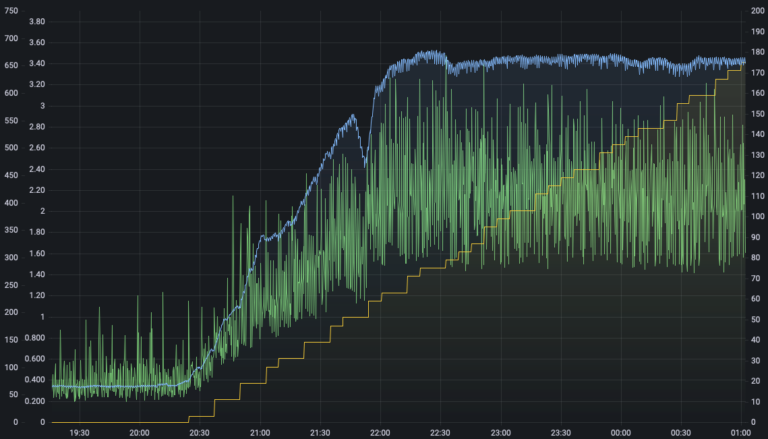
\includegraphics[width=15cm,center]{Figures/cpuValidatorsGossip.png}
    \caption{Graph plots CPU usage (green line, scale up to 3.80 in GHz) and gossip network messages per second (blue line, scale up to 750 messages/sec ), against the number of additional validators being run increase (yellow line, scale up to 200 clients). Source: \cite{Sutton2022ExploringSymphonious}}
    \label{Figure:validatorIncrease}
\end{figure}

As expected, a linear correlation can be seen between the increasing additional validators and the CPU usage, but only up to $\sim$65 validators. However, after the 60-70 validator range, the CPU usage and the amount of gossip messages received level off and seem unaffected by the steadily increasing number of validators. 

In each epoch, 32 randomly selected block proposers propose one block per slot. The remaining validators are assigned to one of the 64 voting committees of one of the 32 slots, where they must attest to (vote on the validity of) a new block being proposed. This is depicted in \fref{Figure:AttestationsDiragram} (\sref{AttestationsLitRev}). Each of these committees publish their attestations into separate gossip channels. These votes are then aggregated and pushed out on specific gossip channels by certain validators chosen to do so. 

Full Nodes that are not running validators will only subscribe to the gossip topics that push out aggregated votes. But with each new validator that is run, it subscribes to a new gossip channel associated with the committee it joins. As there are 64 committees per slot, up to 63 additional validators,  the node has to subscribe to and process more gossip messages. However, past this, there are no new gossip topics left to subscribe to, and the CPU usage and the rate of gossip messages levels off, as shown in \fref{Figure:validatorIncrease}.

To model this behaviour, logarithmic and exponential functions were explored. Through extended experimentation and application of prior mathematical knowledge, it was found that the exponential decay function (increasing form), shown in \eref{eqn: ExpDecayGeneral}, most accurately matches the characteristics desired. Initially, it increases almost linearly at a slow rate before levelling off as more validator clients are run on the node. This is consistent with \fref{Figure:validatorIncrease} that grows almost linearly until 64 validators, after which it levels off. Other sources that support this finding include \cite{Roy2022StakingExchange} and \cite{2021HardwareEthstaker}.

\begin{equation}
    \label{eqn: ExpDecayGeneral}
    \boldsymbol{\mathrm{E(\mathrm{x})} = \mathrm{A} (1-\mathrm{e}^{-\mathrm{k}(\mathrm{x})}) + \mathrm{C}}
\end{equation}

To adapt \eref{eqn: ExpDecayGeneral} to this context, the lower limit or Y-intercept, $\boldsymbol{\mathrm{C}}$, can be set to the energy measurement obtained for running a single validator client on a specific node which is denoted by $\boldsymbol{\mathrm{V_{1}}}$. 
As seen in \fref{Figure:validatorIncrease}, the CPU approaches its maximum capacity as the number of validators approaches 64. Meanwhile, the SSD does not have to work at under a high workload as it has already synchronised a copy of the blockchain when the first validator was run. Hence, the asymptotic upper limit of the graph, $\boldsymbol{\mathrm{A}}$, can be set to $\boldsymbol{\mathrm{\overline{P}}_{TDP}}$ due to the aforementioned reasons in \sref{TDPReasoning}. 
$\boldsymbol{\mathrm{x}}$ denotes the number of additional validator clients run on a node and therefore only takes on positive integer values. This is because the equation has it lower limit set to running a single validator and is designed to account for any validators added after that. 
The growth rate constant $\boldsymbol{\mathrm{k}}$ determines how quickly the energy consumption increases as the validators increase. It can be calculated on a case-by-case basis for any node. 
This equation can be simplified by removing the $\boldsymbol{ + \mathrm{C}}$. It acts as a transition upwards to the graph output by this equation. Removing this transition means we have to subtract $\boldsymbol{ \mathrm{C}}$ from the asymptotic upper-limit $\boldsymbol{\mathrm{\overline{P}}_{TDP}}$ too. Through these modifications emerges an equation for $\boldsymbol{{\mathrm{\overline{V}(\mathrm{x})}}}$ that estimates the extra energy consumed by $\boldsymbol{\mathrm{x}}$ additional validators:

\begin{equation}
    \label{eqn:ExpDecay}
    \boldsymbol{\mathrm{\overline{V}(\mathrm{x})} = \left(\mathrm{\overline{P}}_{TDP} -\mathrm{\overline{V}_{1}} )\right(1-\mathrm{e}^{-\mathrm{k}(\mathrm{x})}) \qquad \forall x \in \mathbb{Z}^+}
\end{equation}

\label{DetermineK}
Below is an example calculation to determine constant $\boldsymbol{\mathrm{k}}$ for a node with hardware configuration 6 (see in \tref{Table:CCRIhardwareConfig}, \sref{ImplementationSection}). 

$\boldsymbol{\mathrm{C}} = \boldsymbol{\mathrm{150.20}} $W, \textbf{assuming} the node runs the most common CL and EL client combination, Prysm and Geth. Mean values are taken from  \cite{CryptoCarbonRatingsInstitute2022TheNetwork}.

$\boldsymbol{\mathrm{A}} = \boldsymbol{\mathrm{280}}$W, the TDP rating for AMD 3970X \cite{AMDDatabase}. When subtracted by the $\boldsymbol{\mathrm{C}}$ value, it equals $\boldsymbol{\mathrm{129.80}}$W.

$\boldsymbol{\mathrm{x}} $ can be set to $\boldsymbol{\mathrm{63}} $ additional validators, as the graph starts at 1 validator running already, totalling 64 validators. Furthermore, this can be equated to $\boldsymbol{\mathrm{0.9 * TDP} = 252}$W through the \textbf{assumption} that the CPU operates at just 10\% below its maximum capacity (TDP rating) at the 63$^\mathrm{{rd}}$ additional validator. Subtraction by $\boldsymbol{\mathrm{C}}$ to account for the upward translation discussed earlier results in $\boldsymbol{\mathrm{252-150.20 = 101.8}}$W. 

\begin{equation*}
    \boldsymbol{\mathrm{129.8} * (1-\mathrm{e}^{-\mathrm{k}(\mathrm{63})}) = \mathrm{101.80}}
\end{equation*}

Which solves to:
\begin{equation*}
    \boldsymbol{\mathrm{k} = \mathrm{{2.435} * {10}^{-2}}}
\end{equation*}

Figure \ref{Figure:MultipleValidators} graphs the example introduced above.

% MultipleValidators graph_________
\begin{figure}[htb!]
    \centering
    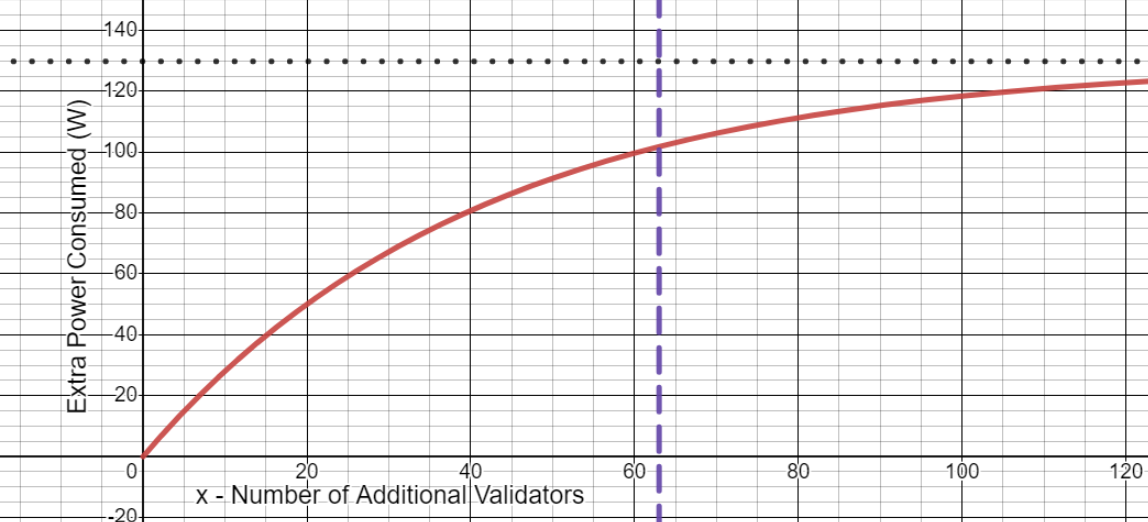
\includegraphics[ width=14cm,center]{Figures/AsymptoteMultipleValidators.png}
    \caption{Graphing \eref{eqn:ExpDecay} showing its inverse exponential decay behaviour, for the hardware configuration 6 example discussed above. The asymptote at $\boldsymbol{\mathrm{A = 129.80}}$W is highlighted by the horizontal dotted (black) line. The dashed vertical (purple) line highlights the value of the curve at $\boldsymbol{\mathrm{x = 63}}$ additional validators to be $\boldsymbol{\mathrm{101.8}}$W.}
    \label{Figure:MultipleValidators}
\end{figure}

\eref{eqn:ExpDecay} is case specific and can be applied independently to estimate the electricity usage of a node with a specific combination of an EL and CL client, as well as a specific hardware configuration. To integrate this equation into the one proposed earlier, \eref{eqn:CCRISync}, it needs to be generalised, keeping all combinations of hardware and clients in mind.

To recapitulate, $\boldsymbol{\mathrm{\overline{V}_{1}}}$ captures the average electricity consumed by a node, running one validator client. 

\begin{equation*}
    \boldsymbol{\mathrm{\overline{V}_{1}} = {\frac{\displaystyle\sum\limits_{i=1}^{n}{ \left({\left(\mathrm{\overline{P}}_{ID} + \mathrm{\overline{P}}_{CL} + \mathrm{\overline{P}}_{EL}\right)} * {\phi_{EL,CL}} \right)}}
{\pi}} }
\end{equation*}

Following this, \eref{eqn:CCRISync} introduced earlier can be re-written as:

\begin{equation*}
     \boldsymbol{\overline{\mathrm{P}}_{SNC} +  \overline{\mathrm{V}}_{1} 
} 
\end{equation*}

When modified to account for $\boldsymbol{\mathrm{x }}$ additional validator clients being run on the same node, it results in 'Model-A' proposed by this study: 

\begin{equation}
\label{eqn:FinalEqnShort}
     \boldsymbol{\mathrm{P}_{SNC} +  \overline{\mathrm{V}}_{1} + \mathrm{\overline{V}(\mathrm{x})}} 
\end{equation}

Which can be expanded to:
\begin{equation*}
     \boldsymbol{\mathrm{P}_{SNC} +  \overline{\mathrm{V}}_{1} + {\left(\mathrm{\overline{P}}_{TDP} -\overline{\mathrm{V}}_{1} )\right(1-\mathrm{e}^{-\mathrm{k}(\mathrm{x})}) \qquad \forall x \in \mathbb{Z}^+}} 
\end{equation*}

Expanding all terms results in the final equation for 'Model-A' to look like:
\begin{align}
\label{eqn:FinalEqnLong}
     &\boldsymbol{({\mathrm{T}_{EL} * ({\mathrm{P}_{TDP}} + \mathrm{P}_{SSD})}) +  {\frac{\displaystyle\sum\limits_{i=1}^{n}{ \left({\left(\mathrm{\overline{P}}_{ID} + \mathrm{\overline{P}}_{CL} + \mathrm{\overline{P}}_{EL}\right)} * {\phi_{EL,CL}} \right)}}
{\pi}}}\nonumber \\  \nonumber\\  
     &\boldsymbol{+ {(\mathrm{\overline{P}}_{TDP} - {\frac{\displaystyle\sum\limits_{i=1}^{n}{ \left({\left(\mathrm{\overline{P}}_{ID} + \mathrm{\overline{P}}_{CL} + \mathrm{\overline{P}}_{EL}\right)} * {\phi_{EL,CL}} \right)}}
{\pi}}} ) (1-\mathrm{e}^{-\mathrm{k}(\mathrm{x})})}\\ \nonumber \\    
     &\boldsymbol{\qquad \qquad \qquad \qquad \qquad \qquad \forall \text{ } x \in \mathbb{Z}^+}\nonumber 
\end{align}

Note that hardware configuration-specific terms, such as the CPU's TDP, SSD's power usage and even electricity measurements for each client, must be weighted by the estimated share of the network using that node hardware in order to get a better estimate for the network's cumulative energy consumption. 

% ___________________________________________________________________MODELS DONE< NOW 

% Model-AAAAAAAAAAAAAAAAAAAAAAAAAAAAAAAAAAAAAAAAAAAAAAAAAA
\section{Results Of Application Of Models And Discussion}
\label{ImplementationSection}
Through extensive data gathering, Model-A, alongside 2 other models from the wider literature, are implemented in this section.


\subsection{Model-A: Implementation}

First, 3 hardware configurations were chosen, including a low, medium and high tier for running Full Nodes. Hardware configurations recommended for running the Geth EL client ($\sim$ 70\% network share) can be found in \tref{Table:RecommendedHardware}.

\begin{table}[htb!]
    \centering
    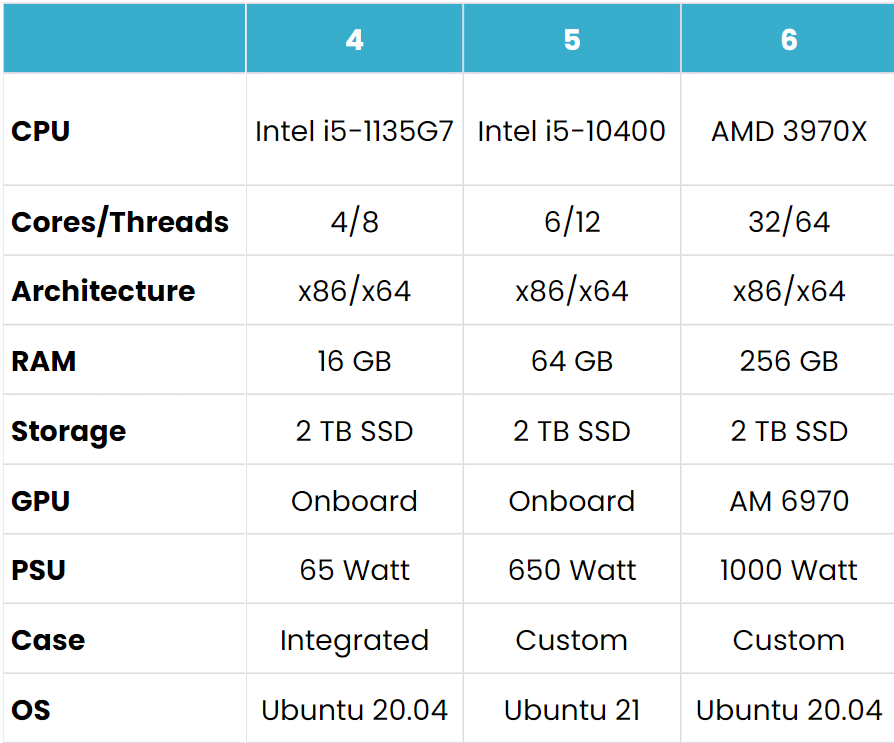
\includegraphics[width=10cm,center]{Figures/CCRIhardwareConfigEdit.png}
    \caption{Adapted from the CCRI report \cite{CryptoCarbonRatingsInstitute2022TheNetwork}, this table shows 3 of the 6 hardware configurations that were used in their experiment detailing a low, mid and high-tier node.}
    \label{Table:CCRIhardwareConfig}
\end{table}

PoS Ethereum was aimed at being run on commodity hardware. Keeping this, as well as the hardware recommendations in \tref{Table:RecommendedHardware} in mind, 3 sets of hardware combinations need to be chosen for implementation of the model. Due to the limited availability of empirical data on hardware running PoS Ethereum, the hardware configurations 4,5 and 6 from \tref{Table:CCRIhardwareConfig} are used. Using this data also helped draw fairer comparisons when evaluating Model-A later on. 

\textit{Step 1 - Average Sync Energy of a Node}

No empirical data was available for implementing the first part of 'Model-A', \eref{eqn:FinalEqnShort}, denoted by $\boldsymbol{\mathrm{P}_{SNC}}$. Non-scientific data gathered on the synchronisation time $\boldsymbol{\mathrm{T}_{EL}}$, reported by users employing varying combinations of hardware and EL clients, can be found in Appendix B. This data is limited and thus insufficient to differentiate between the sync times for the 4 major EL clients. However, it is sufficient to estimate the average sync time of varying tiers of node hardware (relative to \tref{Table:CCRIhardwareConfig}), presented in \tref{Table:SyncEnergy}. Data collected on hardware running the Geth client was \textbf{assumed} to be more representative and given a higher weighting due to its high network share of $\sim$ 70\%. 

Varying external factors affect a user's decision to choose the appropriate hardware for their node, ranging from different profit structures to low-budget devices and future-proof hardware. There is an immeasurable amount of hardware configurations that users could opt for. Thus, we model this distribution of the 3 categories of node hardware using a continuous distribution, particularly - the CDF (Cumulative distribution function) of the standard normal distribution. This distribution was divided into 3 parts; 25\% of the network is \textbf{assumed} to opt for the low-tier hardware (configuration 4), 50\% for the mid-tier (configuration 5) and 25\% for the high-tier hardware (configuration 6), presented in \tref{Table:SyncEnergy}. 

\begin{table}[h]
\centering
\begin{tabular}{|l|l|l|l|l|}
\hline
\textbf{Tier} & \textbf{$\boldsymbol{\mathrm{T}_{EL}}$ {[}h{]}} & \textbf{$\boldsymbol{\mathrm{P}_{TDP}}$ {[}Wh{]}} & \textbf{$\boldsymbol{\mathrm{P}_{SSD}}$ {[}Wh{]}} & \textbf{Share of the network {[}\%{]}} \\ \hline
Low    & 36 & 28  & 3.5 & 25 \\ \hline
Medium & 24 & 65  & 8.5 & 50 \\ \hline
High   & 12 & 280 & 10  & 25 \\ \hline
\end{tabular}
\caption{Data used to implement the  $\boldsymbol{\mathrm{P}_{SNC}}$ part of 'Model-A'.  $\boldsymbol{\mathrm{P}_{TDP}}$ source: \cite{IntelFAQs}, \cite{AMDDatabase}. $\boldsymbol{\mathrm{P}_{SSD}}$ source: \cite{RachanaKhamamkar2020AnalyzingDrives}.}
\label{Table:SyncEnergy}
\end{table} 

Given \tref{Table:SyncEnergy}, the $\boldsymbol{\mathrm{P}_{SNC}}$ for an average node can be calculated by following its \eref{eqn:Sync}. Each hardware tier's values are multiplied by its network distribution share: 
\begin{align}
    &\boldsymbol{0.25*(36*(28 + 3.5)) + 0.5*(24*(65+8.5)) + 0.25*(12*(280+10))} \nonumber\\ \nonumber \\
    &\boldsymbol{{\mathrm{P}_{SNC}} = 2035.5} \text{ Wh per node} \nonumber
\end{align}

% ________________________________________--

% _---------------------------------------
\textit{Step 2 - Average electricity consumption of a node, bar sync energy}
\label{postSyncEnergyImplementation}

The next part of \eref{eqn:FinalEqnShort}, $\boldsymbol{\mathrm{\overline{V}_{1}}}$ needs to be implemented. \tref{Table:ClientShares} presents contemporary data collected for each EL and CL client's shares of the Ethereum network, required to calculate $\boldsymbol{\phi_{EL,CL}}$.  

% --------------------------------------
\begin{table}[h]
    \centering

  \subcaptionbox{\textbf{Execution Clients} \cite{Sigp/blockprint:Metrics}}{
      \begin{tabular}{|l|c|}
            \hline
             Geth & 69.22 \% \\
            \hline
             Nethermind & 14.16 \%  \\
            \hline 
             Erigon & 10.65 \% \\
            \hline
             Besu & 5.78 \% \\
            \hline
             OpenEthereum & 0.00 \% \\
            \hline
             Other & 0.20 \% \\
            \hline
  \end{tabular}
    \label{Table:ClientShares:left}
  }
  \subcaptionbox{\textbf{Consensus Clients}  \cite{ClientsExplorer}}{
        \begin{tabular}{|l|c|}
                    \hline
             Prysm & 65.15 \%  \\
            \hline
             Lighthouse & 29.30 \% \\
            \hline 
             Teku & 10.65 \% \\
            \hline
             Nimbus & 0.91 \% \\
            \hline
             Lodestar & 0.0 \% \\
            \hline
             Other & 0.0 \%  \\
            \hline
            
  \end{tabular}
    \label{Table:ClientShares:right}
  }
    \caption{An updated table of client diversity within Ethereum Mainnet network, data recorded on 27-Mar 23. Updates table 5 from report \cite{CryptoCarbonRatingsInstitute2022TheNetwork} }
  \label{Table:ClientShares}
\end{table}

% --------------------------------------------


Empirical data on the energy consumption values recorded for all 3 hardware configurations running all clients separately can be found in \tref{Table:ConsumptionValues}. The Nethermind client which now holds a sizeable network share has no empirical energy consumption data available. Its values are substituted by the other 3 EL clients' averaged values per configuration.

% ----------------------
\begin{table}[htb!]
\centering
\begin{tabular}{|l|lll|}
\hline
\textbf{Client Name} & \multicolumn{3}{l|}{\textbf{Node Configuration}}                               \\ \hline
\textbf{}            & \multicolumn{1}{l|}{\textbf{4}} & \multicolumn{1}{l|}{\textbf{5}} & \textbf{6} \\ \thickhline
Idle Node (No Client)               & \multicolumn{1}{l|}{3.66}       & \multicolumn{1}{l|}{25.04}      & 78.17      \\ \cline{1-1}
Geth (EL)            & \multicolumn{1}{l|}{11.23}      & \multicolumn{1}{l|}{9.70}       & 47.70      \\ \cline{1-1}
Erigon (EL)          & \multicolumn{1}{l|}{18.60}      & \multicolumn{1}{l|}{17.59}      & 44.62      \\ \cline{1-1}
Besu (EL)            & \multicolumn{1}{l|}{30.25}      & \multicolumn{1}{l|}{31.02}      & 75.04      \\ \cline{1-1}
Nethermind(EL)[Averaged] & \multicolumn{1}{l|}{20.03}       & \multicolumn{1}{l|}{19.44}       & 55.79      \\ \cline{1-1}
Prysm (CL)           & \multicolumn{1}{l|}{3.51}       & \multicolumn{1}{l|}{2.87}       & 24.33      \\ \cline{1-1}
Lighthouse (CL)      & \multicolumn{1}{l|}{2.75}       & \multicolumn{1}{l|}{3.14}       & 18.84      \\ \cline{1-1}
Teku (CL)            & \multicolumn{1}{l|}{3.71}       & \multicolumn{1}{l|}{3.32}       & 27.46      \\ \cline{1-1}
Nimbus (CL)          & \multicolumn{1}{l|}{1.67}       & \multicolumn{1}{l|}{2.08}       & 17.11      \\ \cline{1-1}
Lodestar(CL)         & \multicolumn{1}{l|}{3.14}       & \multicolumn{1}{l|}{3.89}       & 33.55      \\ \hline

\end{tabular}
\caption{Mean electricity consumption values [in Wh] measured in the report \cite{CryptoCarbonRatingsInstitute2022TheNetwork} for hardware configurations 4-6 mentioned in \tref{Table:CCRIhardwareConfig} running various clients.  }
\label{Table:ConsumptionValues}
\end{table}

Given the data in \tref{Table:ConsumptionValues}, values in \tref{Table:EstimatesPerNode} were be calculated. For example, the first row (Prysm,Geth) was calculated by adding the electricity usage when idle, running Pyrsm, and running Geth per configuration, multiplied by its hardware tier distribution across the network, shown below:
\begin{align}
    &\boldsymbol{0.25*(3.66 + 11.23 + 3.51) + 0.50 * (25.04 + 9.70 + 2.87) + 0.25} \nonumber\\
    &\boldsymbol{* (78.17 + 47.70 + 24.33) = 60.96}\text{Wh} \nonumber
\end{align}

% -----------------------------------------
\begin{table}[htb!]
\centering
\begin{tabular}{|ll|l|l|l|}
\hline
\multicolumn{2}{|l|}{\textbf{Client Combination}} &
  \multirow{2}{*}{\textbf{\begin{tabular}[c]{@{}l@{}}Estimate\\ {[}Wh{]}\end{tabular}}} &
  \multirow{2}{*}{\textbf{\begin{tabular}[c]{@{}l@{}}Annualised Estimate\\ {[}kWh/year{]}\end{tabular}}} &
  \multirow{2}{*}{\textbf{\begin{tabular}[c]{@{}l@{}}Client Combination\\ Share {[}\%{]}\end{tabular}}} \\ \cline{1-2}
\multicolumn{1}{|l|}{\textbf{CL Client}} & \textbf{EL Client} &       &        &       \\ \hline
\multicolumn{1}{|l|}{Prysm}              & Geth               & 60.96 & 533.97 & 45.10 \\ \cline{1-2}
\multicolumn{1}{|l|}{Prysm}              & Erigon             & 65.97 & 577.91 & 6.94  \\ \cline{1-2}
\multicolumn{1}{|l|}{Prysm}              & Besu               & 83.21 & 728.88 & 3.77  \\ \cline{1-2}
\multicolumn{1}{|l|}{Prysm}              & Nethermind         & 70.05 & 613.62 & 9.23  \\ \cline{1-2}
\multicolumn{1}{|l|}{Lighthouse}         & Geth               & 59.53 & 521.47 & 20.28 \\ \cline{1-2}
\multicolumn{1}{|l|}{Lighthouse}         & Erigon             & 64.54 & 565.41 & 3.12  \\ \cline{1-2}
\multicolumn{1}{|l|}{Lighthouse}         & Besu               & 81.78 & 716.38 & 1.69  \\ \cline{1-2}
\multicolumn{1}{|l|}{Lighthouse}         & Nethermind         & 68.62 & 601.11 & 4.15  \\ \cline{1-2}
\multicolumn{1}{|l|}{Teku}               & Geth               & 62.01 & 543.24 & 7.37  \\ \cline{1-2}
\multicolumn{1}{|l|}{Teku}               & Erigon             & 67.03 & 587.18 & 1.13  \\ \cline{1-2}
\multicolumn{1}{|l|}{Teku}               & Besu               & 84.26 & 738.15 & 0.62  \\ \cline{1-2}
\multicolumn{1}{|l|}{Teku}               & Nethermind         & 71.11 & 622.88 & 1.51  \\ \cline{1-2}
\multicolumn{1}{|l|}{Nimbus}             & Geth               & 58.29 & 510.66 & 0.63  \\ \cline{1-2}
\multicolumn{1}{|l|}{Nimbus}             & Erigon             & 63.31 & 554.59 & 0.10  \\ \cline{1-2}
\multicolumn{1}{|l|}{Nimbus}             & Besu               & 80.54 & 705.57 & 0.05  \\ \cline{1-2}
\multicolumn{1}{|l|}{Nimbus}             & Nethermind         & 67.39 & 590.31 & 0.13  \\ \hline
\end{tabular}
\caption{Electricity consumption estimates (best guess) per node for all possible client combinations. Used to calculate $\boldsymbol{\mathrm{\overline{V}_{1}}}$.  }
\label{Table:EstimatesPerNode}
\end{table}

% -----------------------------------
Following \eref{eqn:CCRI}, best guess for an individual node =  \textbf{63.76 Wh}. This can be annualised (8760h in a year) = \textbf{558.55 kWh/year}.

\textbf{Assuming} the node needs to perform a fresh synchronisation once a year, the annual total consumption of an average node (running 1 validator):

\begin{align}
    &\boldsymbol{ \mathrm{\overline{V}_{1}} + \mathrm{P}_{SNC} = \text{560.58 kWh/year or 63.99 Wh.}} \nonumber
\end{align} 

% --------------------------------------------------
% STAGE 3 of implementation with multiple validators
% --------------------------------------------------
\textit{ Step 3 - Operating additional validators on some nodes}

Implementing the final part of \eref{eqn:FinalEqnShort}, $\boldsymbol{\mathrm{\overline{V}(\mathrm{x})}}$, accounts for some nodes running multiple validators. 

When users operate additional validator clients, they often run a 1000+ to take advantage of the exponential decrease in energy consumption, seen in \sref{AdditonalNodesReasoning}. Currently, there are 561,472 validators running. Based on this, and for the sake of simplicity, it can be \textbf{assumed} that 1000 additional validators are run on $\sim$562 nodes (of the total $\sim$12000 network nodes), running on mid to high-tier hardware. Thus, following \eref{eqn:Sync} yields:

$\boldsymbol{\mathrm{\overline{P}}_{TDP}}$ (from \tref{Table:SyncEnergy}): \textbf{205 Wh} \\
$\boldsymbol{ \overline{\mathrm{V}}_{1}}$ (from \sref{postSyncEnergyImplementation}) : \textbf{63.99 Wh} 

$\boldsymbol{\mathrm{k}}$ can be calculated by the method shown in the example in \sref{DetermineK}:

\begin{equation*}
    \boldsymbol{\mathrm{141.01} * (1-\mathrm{e}^{-\mathrm{k}(\mathrm{63})}) = \mathrm{120.51}}
\end{equation*}

Which solves to:
\begin{equation*}
    \boldsymbol{\mathrm{k} = \mathrm{{3.061} * {10}^{-2}}}
\end{equation*}

Once $\boldsymbol{\mathrm{k}}$ has been calculated, $\boldsymbol{\mathrm{x}}$ can be set to \textbf{1000} additional validators for 562 of the total nodes on the network while the rest run no additional nodes.
\begin{center}
    $\boldsymbol{\mathrm{\overline{V}(\mathrm{1000})}} =$ \textbf{141.10 Wh} \\
 \textbf{141.10 $*$ 562 = 79.29 kWh}
\end{center}

The new hourly consumption of the entire network: \textbf{862.66 kWh}. Final results are compiled in \tref{Table:FinalResults}.
% The new hourly energy consumption of a single node can be derived: \textbf{70.47} Wh
% Annual energy consumption of a single node: 617.30 kWh 
% Annual energy consumption of the network: 7.5569 GWh
% Annual energy consumption of a single node per transaction: 0.0015738 Wh/tx
% Annual energy consumption of the network per transaction: 19.27 Wh/tx



% ____________________________________________________________________________
% \subsubsection{Additonal Assumptions}
% \label{Assumptions}

% \begin{itemize}
    % \item They have taken the syncing on nodes into account into their model whereas for general modelling, it would be  abetter estimate to ignore this initial set up energy and get an avergae form then on. That is what this paper has done, taking averages of the Raspberry Pi rather than including the syncing energy.
    % \item The TDP + SSD power usage can be used as an upper limit for the energy consumption of any hardware set-up
    % \item That growth for more than one validator can be modelled by an exponential decay (increasing form)
    % \item This exponential growth has an upper limit of TDP + SSD power usage and using the single validator energy consumption as the lower limit
%     \item The CCRI model has been verified and is accurate. Thus it is acceptable to use as the base for 'Model-A'
%     \item The EL and CL clients are not changed; just additional Validator clients are run on the same set up
%     \item 10\% lower than the TDP power should be reached by the time the 64$^\mathrm{{th}}$ validator is run.
%     \item Took averages of other EL layer clients per confirguration for NetherMind. not good.
%     \item All these numbers are for running a full node, not validators which sdmieler,2020 said is basically negligible
%     \item high, mid low tiers dont have a fair distribution of hardware but does help achieve more accurate results hopefully
%     \item for table \_\_ gave higher importance to Geth to estimate sync time as it has a much larger share of the network than the other EL clients
% \end{itemize}

\subsection{Implementing Competing Models}

As mentioned in \sref{LitRevExistingModels} there are two existing models found in the wider literature. 

\textit{The CCRI Model} 

This model \cite{CryptoCarbonRatingsInstitute2022TheNetwork} forms the $ \boldsymbol{\overline{\mathrm{V}}_{1}}$ part of Model-A proposed in this study, detailed in \sref{CCRIBaseEqnSection}. Through the implementation of Model-A, the \textit{CCRI model} was also implemented as a step. All the contemporary data collected in \tref{Table:ClientShares} and \tref{Table:ConsumptionValues} was used for calculations in \tref{Table:EstimatesPerNode}. Ever since the CCRI report, OpenEthereum has been deprecated, and the Lodestar client no longer holds a sizeable share of the network, and they were not included in calculations. The study splits the network share between the 3 hardware tiers (low, mid and high-tier) binomially rather than using a continuous distribution like this study. However, the split remains the same at 25\%, 50\%, and 25\%, respectively, making the results more comparable. The final results from this model can be found in \tref{Table:FinalResults}.

\textit{The UCL Model} 

The original \textit{UCL Model} can be found in report \cite{Platt2022TheProof-of-Work}. It was recently updated on 7$\mathrm{^{th}}$ Feb 2023 \cite{IbanezTheExpansion}, and contemporary results from the updated report are directly taken and updated with the same metrics used to implement Model-A for a fair comparison. Results can be found in \tref{Table:FinalResults}. 


\subsection{Final Results}
\label{ResultsSection}
Metrics recorded on 10$\mathrm{^{th}}$ April 2023: \\
Number of nodes connected to Ethereum mainnet: \textbf{12242 nodes} \cite{NodewatchAnalytics} \\
Number of transactions completed each day: \textbf{1074596 tx/day}  \cite{EthereumBlockchair} \\
The number of validators on the network: \textbf{562729 validators} 
\cite{EthereumEthereum.orgc}

Using these metrics, results for each of the aforementioned models are presented in \tref{Table:FinalResults}.
% \clearpage
% -----------------------------------------------
% RESULTS  TABLEEEE
% ----------------------------------------------------------------
\begin{table}[htb]
\begin{tabular}{ll"ll"l"l|}
\cline{3-6}
 &
   &
  \multicolumn{2}{l"}{\textbf{Model-A}} &
  \textbf{CCRI \cite{CryptoCarbonRatingsInstitute2022TheNetwork}} &
  \textbf{UCL \cite{IbanezTheExpansion}} \\ \thickhline
\multicolumn{1}{|l|}{\multirow{2}{*}{\textbf{\begin{tabular}[c]{@{}l@{}}Accounts \\ For:\end{tabular}}}} &
  \textbf{\begin{tabular}[c]{@{}l@{}}Synchronisation \\ Energy \end{tabular}} &
  \multicolumn{1}{l|}{Yes} &
  Yes &
  No &
  No \\ \cline{2-6} 
\multicolumn{1}{|l|}{} &
  \textbf{\begin{tabular}[c]{@{}l@{}}Additional Validators \\ Per Node\end{tabular}} &
  \multicolumn{1}{l|}{No} &
  Yes &
  No &
  No \\ \hline
\multicolumn{1}{|l|}{\multirow{2}{*}{\textbf{Hourly}}} &
  \textbf{\begin{tabular}[c]{@{}l@{}}Per Node \\ {[}Wh{]}\end{tabular}} &
  \multicolumn{1}{l|}{63.99} &
  70.47 &
  63.76 &
  85.03 \\ \cline{2-6} 
\multicolumn{1}{|l|}{} &
  \textbf{\begin{tabular}[c]{@{}l@{}}Entire Network \\ {[}kWh{]}\end{tabular}} &
  \multicolumn{1}{l|}{783.37} &
  862.66 &
  780.57 &
  1040.09 \\ \hline
\multicolumn{1}{|l|}{\multirow{4}{*}{\textbf{Annual}}} &
  \textbf{\begin{tabular}[c]{@{}l@{}}Per Node \\ {[}kWh{]}\end{tabular}} &
  \multicolumn{1}{l|}{560.58} &
  617.30 &
  558.55 &
  744.86 \\ \cline{2-6} 
\multicolumn{1}{|l|}{} &
  \textbf{\begin{tabular}[c]{@{}l@{}}Entire Network \\ {[}GWh{]}\end{tabular}} &
  \multicolumn{1}{l|}{6.86} &
  7.56 &
  6.84 &
  9.12 \\ \cline{2-6} 
\multicolumn{1}{|l|}{} &
  \textbf{\begin{tabular}[c]{@{}l@{}}Per Node / Transaction \\ {[}mWh/tx{]}\end{tabular}} &
  \multicolumn{1}{l|}{1.43} &
  1.57 &
  1.42 &
  1.90 \\ \cline{2-6} 
\multicolumn{1}{|l|}{} &
  \textbf{\begin{tabular}[c]{@{}l@{}}Entire Network / Transaction \\ {[}Wh/tx{]}\end{tabular}} &
  \multicolumn{1}{l|}{17.50} &
  19.27 &
  17.43 &
  23.25 \\ \hline
\end{tabular}
\caption{Best guess estimates obtained by implementing 'Model-A' as well as 2 other models, all using the same metrics introduced earlier.}
\label{Table:FinalResults}
\end{table}
% -----------------------------------------------------------------------

% ______________________________________________________________________
% \section {Modelling Ethereum's Carbon Emissions}
% \url{https://ethernodes.org/countries}

% \paragraph{ Simple Linear Regression Model}
% A simple logical model for estimating the energy consumption of Ethereum 2.0's energy consumption logically would be using simple regression. y = mx + c, and if we wanted to say that energy is dependent on transactions, then we can say y is the energy per node, m is the slope we need to find, x is the number of transactions/sec, c is the base energy an idle node requires. Then we multiply this whole thing by the number of validators on the network to get the overall network energy consumption.

% _____________________________________________________________________________
% _____________________________________________________________________________
% ____________________________________________________________________________
\section{Evaluation and Discussion}

\subsection{Interpretation}

Being able to model the electricity consumption of PoS Ethereum successfully answers RQ1. The results produced by Model-A are valid due to three main reasons:
\begin{enumerate}
    \item The qualitative criteria defined in \sref{QualModelEvalMEthodology}, for model formulation to be valid, has been met. 
    \begin{itemize}
        \item Credible sources have been used to justify each assumption and conclusion drawn during the formulation of Model-A. Comprehensive documentation of each justification has been provided, and all 8 assumptions have been emphasised in the text using bold formatting.
        \item All data utilised in the modelling process were either derived from strictly empirical sources or an average of a comprehensive collection of non-scientific sources.
    \end{itemize}
    \item Model-A's results fall between the only two other models found in the wider literature, thus positioning them within a 'reasonable' range.
    \item In accordance with the quantitative evaluation criteria defined in \sref{MethoologyErrorQuant}, for the results to be deemed satisfactory, $\boldsymbol{\epsilon_\mathrm{rme} \leq 0.2}$. By treating the experimentally verified \textit{CCRI model's} results as true values and comparing the energy consumption for the entire network per transaction, the $\boldsymbol{\epsilon_\mathrm{rme} = 7.96 * 10^{-2}}$ is obtained, making it acceptable.   
\end{enumerate}

Model-A accounts for 2 more sources of energy expenditure as compared to the base \textit{CCRI model}, which explains the average Percentage Increase (PE) of 9.5\% across all values. 9.25\% of it can be attributed to operating additional validators, suggesting that the extra energy consumed by accounting for $\sim$500000 extra validators was weighted reasonably since it didn't have a disproportionate effect on Model-A's final results. 

The \textit{UCL model} seems to overestimate consumption values. This may stem from the model's lack of complexity, which is a consequence of its generalisation to encompass six PoS blockchains.

\begin{figure}[!htb]
    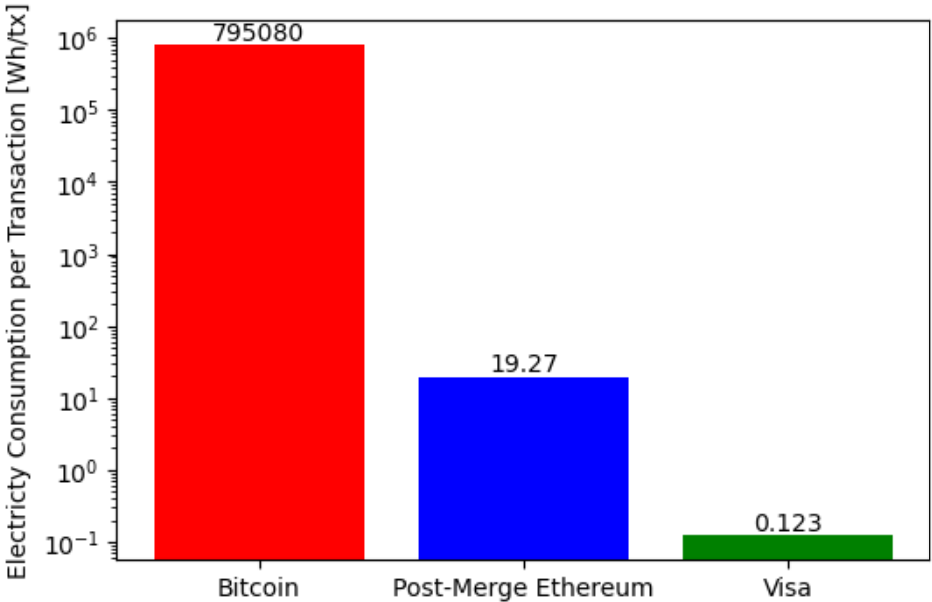
\includegraphics[width=13cm,center]{Figures/ElectricityConsumptionPlot.png}
    \caption{2022 data on electricity consumption per transaction for Bitcoin \cite{BitcoinDigiconomist}, Ethereum 2.0 [from Model-A] and Visa \cite{2022VisaReport}, \cite{VisaHome} plotted on a logarithmic scale. Code available in Appendix C.}
    \label{Figure:ElectricityConsumptionPlot}
\end{figure}

PoS Ethereum has had a reduction of 99.997\% in its overall energy use when compared to PoW Ethereum's consumption average over 2022, going from 24.99TWh/year to 7.56kWh/year according to Model-A \cite{CCRIIndices}. This answers RQ2 (\sref{ResearchQuestions}) - the claimed energy reduction figure, 99.988\%, is only inaccurate by less than 0.01\% according to Model-A, as shown in \fref{Figure:PaypalEthElectrcityPlot}.

According to \fref{Figure:ElectricityConsumptionPlot}, Visa can process 
$\sim$156 transactions in the same amount of energy it takes PoS Ethereum to complete a single one. This often-made comparison is not one that is fair to make. Ethereum is a completely self-contained monetary system, whereas Visa relies on a range of intermediaries such as the global banking system, SWIFT and the diplomatic strength of the U.S. government \cite{Carter2021BitcoinComparison}. Thus, they are dissimilar in nature. Instead, Ethereum should be compared to Paypal, a platform that, along with digital payments, also offers other financial services and bank-like services.  

\begin{figure}[!htb]
    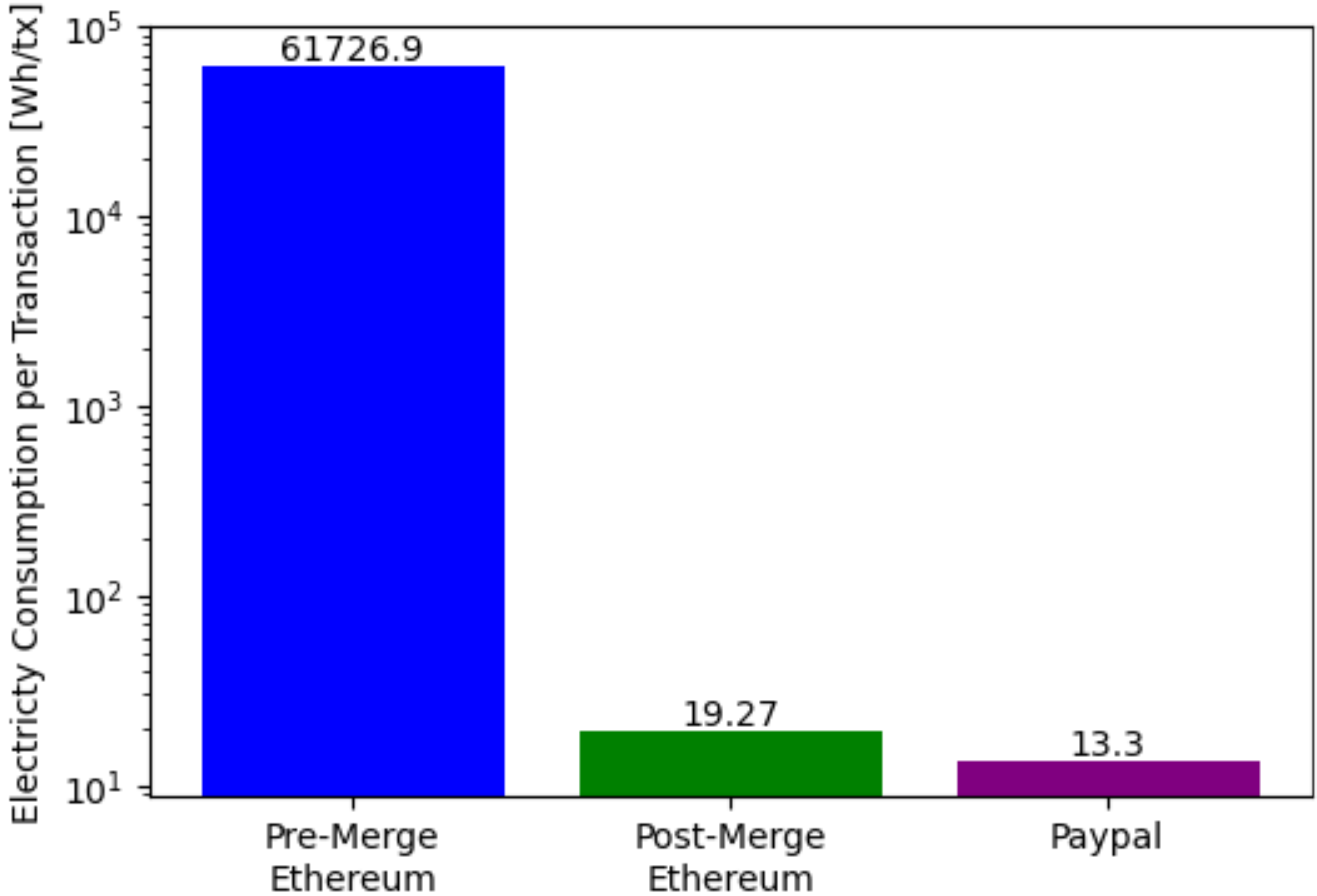
\includegraphics[width=13cm,center]{Figures/PaypalEthElectrcityPlot.png}
    \caption{Electricity consumption per transaction for Ethereum 1.0 \cite{CCRIIndices}, \cite{EthereumBlockchair}, Ethereum 2.0 [from Model-A] and Paypal \cite{2007IntroductionPayPal}. Code found in Appendix C.}
    \label{Figure:PaypalEthElectrcityPlot}
\end{figure}

\fref{Figure:PaypalEthElectrcityPlot} shows that Ethereum 2.0 is impressively close to Paypal's energy consumption while maintaining decentralisation, according to Model-A.



% ____________________________________________________________________________
\subsection{Limitations and Future Work}
\label{LimitationsFutureWork}

\textbf{Secondary data:} Data from the scientific experiment performed in the CCRI report \cite{CryptoCarbonRatingsInstitute2022TheNetwork} was used as it measured the precise metrics needed for this study. First-hand data collection was out of the scope of this study as the hardware required for mid and high-tier configurations would've cost $\sim$£2500 while also requiring 23 days of simultaneously running all 3 nodes. However, no validator nodes were run in the experiment as staking 32ETH was infeasible and the additional electricity was viewed as negligible. While we have disproven this assumption by modelling data found from consistent but non-scientific sources, more work is needed on studying the effects of overloading nodes with thousands of additional validators. Moreover, the impact of this workload on different hardware configurations should also be considered so fewer assumptions are made. 

\textbf{Lack of data:} Due to the innovative nature of the research being conducted, there was a paucity of data available for analysis. Some of the improvements made upon the base model come from modelling non-scientific data; hence the model was implemented on averaged values to obtain a 'best guess' estimation. Through further scientific experimentation, high and low estimates can be found to obtain a range that the final results should lie within. 

\textbf{Energy inefficiencies: } Electricity consumption data comes from monitoring software run on computers. Thus, these are not 'at-wall' values which truly show how much electricity is being drawn from the national grid, possibly due to voltage regulators that limit the power supply to the machine. This model could benefit from further work conducted by individuals well versed in electrical engineering that account for this dissipated energy, obtaining a more accurate estimation 'At-wall' \cite{Warkozek2012ACenters}.

\textbf{Simulation and Prediction: } There is potential for future work in creating a computer-based simulation of this model or on existing blockchain benchmarking software such as Hyperledger Caliper or Blockbench \cite{Aldweesh2020BenchmarkingApplications}. A more ambitious goal would be predicting energy consumption,  given the different values for the factors included in the model, which would require curve-fitting \cite{IbanezTheExpansion}.

% _______________________________________________________________________
